\documentclass[10pt,a4paper]{article}
\usepackage[utf8]{inputenc}
\usepackage[T1]{fontenc}
\usepackage{lmodern}
\usepackage[margin=1.5cm, top=1.4cm, bottom=1.4cm]{geometry}
\usepackage{hyperref}
\usepackage{enumitem}
\usepackage{titlesec}
\usepackage{xcolor}
\usepackage{graphicx}

\definecolor{accent}{HTML}{00686E}
\hypersetup{colorlinks=true, urlcolor=accent, linkcolor=accent}
\pagenumbering{arabic}
\setlength{\parindent}{0pt}

\titleformat{\section}{\large\bfseries\color{accent}}{}{0em}{}[\vspace{-0.6em}\rule{\textwidth}{0.8pt}]
\titlespacing{\section}{0pt}{7pt}{4pt}

\newcommand{\role}[4]{%
  \textbf{#1} \hfill \textbf{#2}\\[1pt]%
  \textit{#3} \hfill \textit{#4}\\[2pt]%
}
\setlist[itemize]{leftmargin=1.2em, itemsep=1.5pt, topsep=2pt, parsep=0pt}

\begin{document}

% ================= HEADER =================
\begin{minipage}[c]{0.80\textwidth}
  {\Huge\bfseries Prabhavit Gupta}\\[3pt]
  {\color{accent}\large Media Monitoring Automation Specialist: Workflow Orchestration \& Data Pipelines}\\[6pt]
  {\footnotesize +39 351 610 7807 ~$\vert$~
  \href{mailto:prabhavitg@gmail.com}{prabhavitg@gmail.com} ~$\vert$~
  \href{https://www.linkedin.com/in/prabhavit/}{linkedin.com/in/prabhavit} ~$\vert$~
  \href{https://github.com/prab-gupta}{github.com/prab-gupta} ~$\vert$~
  Venice, Italy (CET Time Zone / EU Permanent Resident)}
\end{minipage}\hfill
\begin{minipage}[c]{0.18\textwidth}
  \raggedleft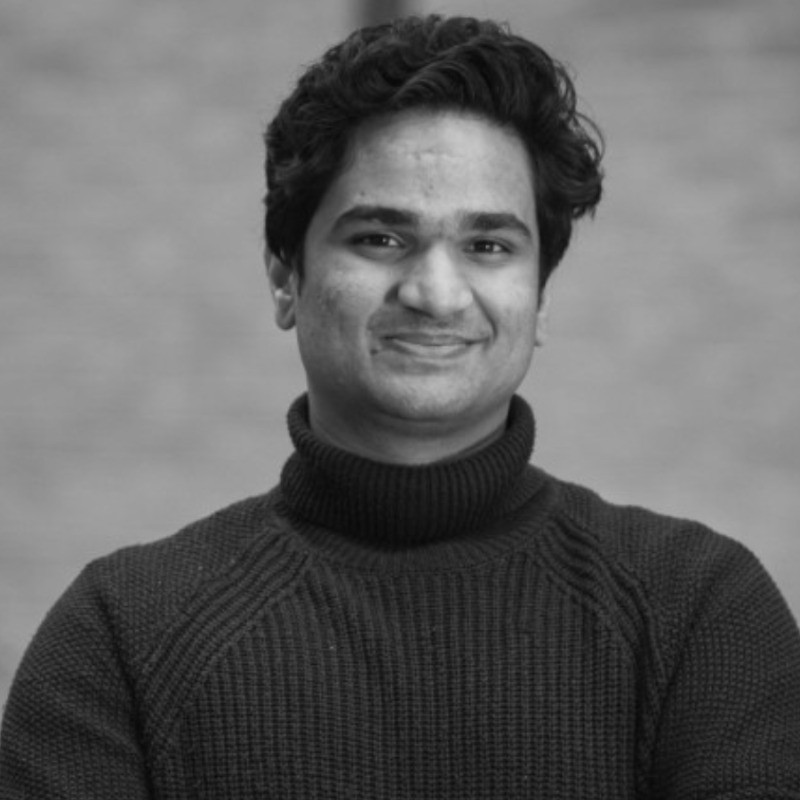
\includegraphics[width=2.0cm]{photo.jpg}
\end{minipage}
\vspace{-2pt}

% ================= SUMMARY =================
\section{Summary}
Automation and Data Pipeline Specialist with 3 years of commercial production experience converting manual content monitoring and extraction processes into scalable, automated workflows. Proven track record architecting event-driven web scraping pipelines, structured document parsing routines, and automated quality verification checks using Python, TypeScript, RESTful webhooks, and modern LLM APIs. Detail-oriented systems builder experienced managing data acquisition pipelines and ensuring consistent delivery quality across global services. Based in Venice, Italy (CET time zone) with an EU Long-Term Residence Permit (permanent unrestricted EU work authorization, no sponsorship required); available immediately for full-time remote roles.

% ================= TECHNICAL EXPERTISE =================
\section{Technical Expertise}
\begin{itemize}
  \item \textbf{Workflow Automation \& Orchestration:} Scalable workflow configuration, transitioning manual processes to automation, n8n, event-driven webhooks, scheduled cron jobs, queue-based pipeline routing (Redis).
  \item \textbf{Media Monitoring \& Content Extraction:} Web scraping (Playwright, BeautifulSoup), full-text extraction, RSS/news feeds, unstructured text parsing, sentiment and entity classification with LLMs.
  \item \textbf{Software Development \& Scripting:} Python (asyncio, pandas, NumPy, requests), TypeScript, Node.js, regex pattern matching, structured JSON schema validation.
  \item \textbf{Data Management \& Quality Control:} PostgreSQL data normalization, automated anomaly detection, deduplication, audit trails, and data provenance verification.
  \item \textbf{DevOps \& Monitoring:} Docker containerization, Git version control, CI/CD pipeline automation, error tracking, automated alert notifications.
  \item \textbf{Languages \& Authorization:} English (C1 Professional, fluent), Hindi (Native), Italian (Conversational). EU Long-Term Residence Permit (unrestricted EU work authorization across all EU member states, no sponsorship required).
\end{itemize}

% ================= EXPERIENCE =================
\section{Experience}

\role{\href{https://flowspace.co}{FlowSpace.co}}{Mar 2024 - Aug 2026}{Lead Developer \& Automation Systems Architect}{London, UK (remote)}
\begin{itemize}
  \item Transitioned manual partner data onboarding into fully automated ingestion and monitoring workflows, processing unstructured data from 4,500+ active enterprise accounts.
  \item Developed automated web extraction and monitoring routines using Playwright and Python, detecting external catalog changes and triggering automated updates.
  \item Implemented automated LLM-based categorization and extraction pipelines, converting unstructured text into normalized database records.
  \item Engineered asynchronous task processing queues using Redis to handle high-volume data streams without impacting real-time user query performance.
  \item Built automated monitoring dashboards and error alerting to ensure data integrity, pipeline throughput, and immediate anomaly notification.
\end{itemize}

\role{Urlink}{Apr 2025 - Jul 2025}{Project Manager \& Solutions Developer (Freelance)}{Barcelona, Spain (remote)}
\begin{itemize}
  \item Led technical workflow design and delivery of automated data synchronization services connecting third-party analytics endpoints to centralized PostgreSQL databases.
  \item Configured automated validation scripts and integration health checks to verify data quality and reduce synchronization latency.
  \item Designed operational documentation and workflow runbooks to support continuous pipeline maintenance.
\end{itemize}

\role{Independent Technical Consultant}{Aug 2023 - Feb 2024}{Automation \& Workflow Developer}{Venice, Italy}
\begin{itemize}
  \item Built and deployed custom automated content monitoring and reporting pipelines for European SMBs using Python and n8n.
  \item Replaced repetitive manual reporting workflows with automated email and Slack digest delivery pipelines.
  \item Authored technical workflow documentation and user guides for non-technical operations teams.
\end{itemize}

% ================= EDUCATION =================
\section{Education}
\role{Ca' Foscari University of Venice}{2020 - 2024}{BA in Philosophy, International Studies and Economics}{Venice, Italy}
\begin{itemize}
  \item Rigorous training in formal logic, analytical problem solving, systems analysis, and macroeconomic decision models.
\end{itemize}

\end{document}
